\documentclass{beamer}

\usepackage[utf8]{inputenc}
\usepackage{subfig}
\usepackage{ngerman}
\usetheme{focus}

% Captions
\usepackage{caption}
\captionsetup[figure]{labelformat=empty}

% Bibliography
\usepackage[citestyle=numeric,style=numeric,backend=biber]{biblatex}
\addbibresource{bibliography.bib}

\title{Prozedurale Generierung\\ von Wirbeltierskeletten}
\author{Nina Zimbel}
\institute{KIT - Institut für Visualisierung und Datenanalyse}
\date{7.\ Juli 2020}

% Shorcuts
\newcommand{\zb}{z.\,B.\ }
\newcommand{\dash}{d.\,h.\ }
\newcommand{\va}{v.\,a.\ }
\newcommand{\ua}{u.\,a.\ }
\newcommand{\bzw}{bzw.\ }
\newcommand{\etc}{etc.\ }

\begin{document}

\begin{frame}
 \maketitle
\end{frame}

%-------------------
%\section{Einleitung}
%-------------------
\begin{frame}[focus]
 \begin{figure}
  \centering
  \includegraphics[width=\textwidth]{graphics/kaninchen.jpg}
  \caption{Skelett eines Kaninchens \cite{Spezielle_Zoologie}}
 \end{figure}
\end{frame}

\begin{frame}[focus]
 \begin{figure}
  \centering
  \includegraphics[width=\textwidth]{graphics/ziva-post2.jpg}
  \caption{Maya Plugin Ziva, wirklichkeitsgetreues Modell eines Löwen \cite{Ziva_Lion}}
 \end{figure}
\end{frame}

\begin{frame}[plain]
 \begin{figure}
  \centering
  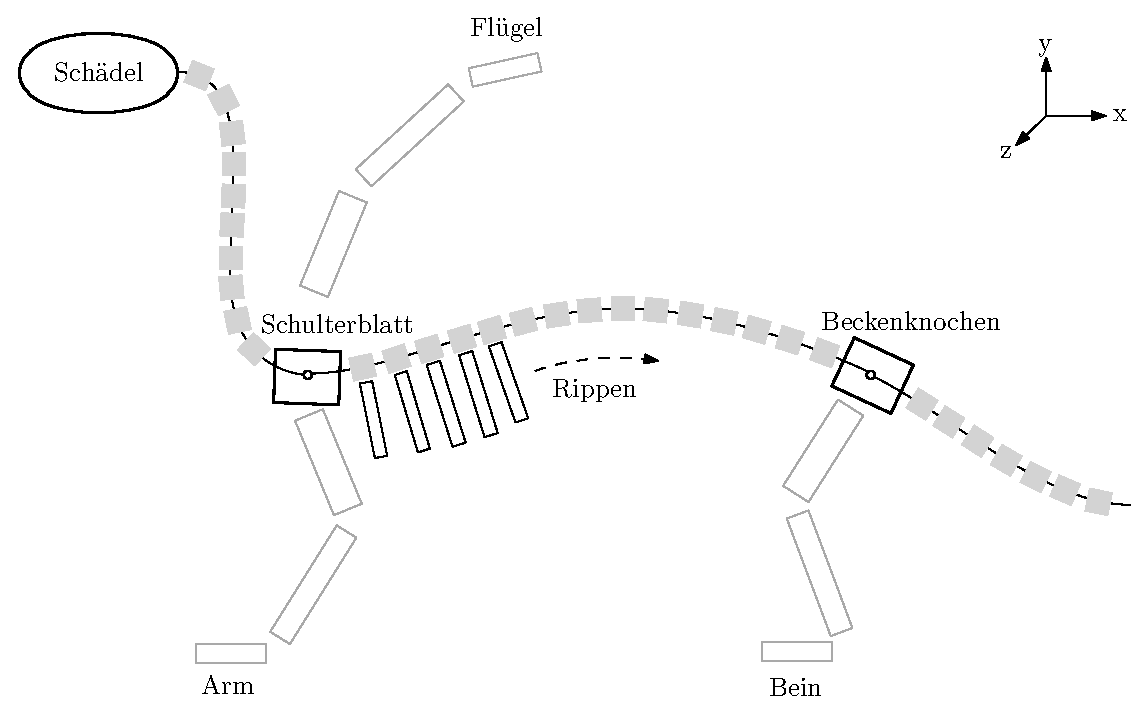
\includegraphics[width=\textwidth]{../graphics/skeletonPlan}
  \caption{Abstrahierter Grundbauplan eines Wirbeltierskeletts}
 \end{figure}
\end{frame}

%-------------------------------------
\section{Principal Component Analysis}
%-------------------------------------
\begin{frame}{PCA}
 \begin{minipage}{0.6\textwidth}
   \begin{itemize}
    \item Gegeben: Menge normalverteilter $n$-dimensionaler Punkte
    \item Gesucht: Achsen des Hyperellipsoids $\rightarrow$ Basis des \emph{Konfigurationsraums}, der durch diese Achsen aufgespannt wird
  \end{itemize}
 \end{minipage}~
 \begin{minipage}{0.4\textwidth}
  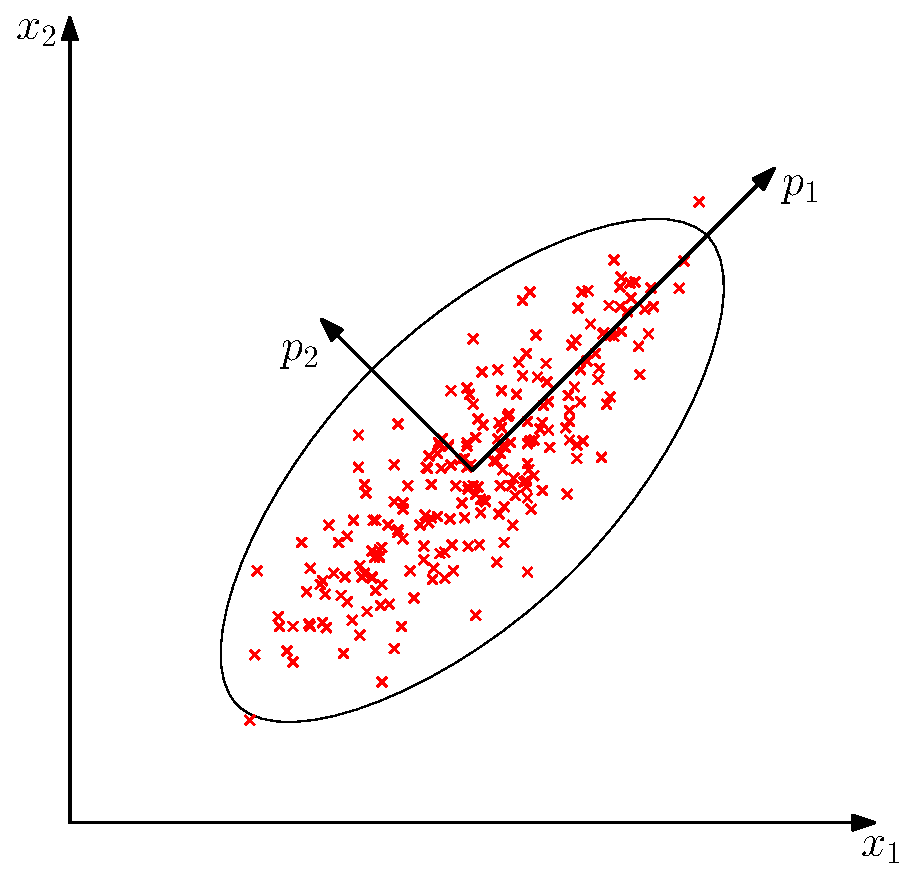
\includegraphics[width=\textwidth]{graphics/pca}
 \end{minipage}
 
 \begin{itemize}
  \item Verteilungen entlang der Achsen sind unabhängig voneinander $\rightarrow$ Erzeugung zufälliger Punkte mit gleicher Verteilung wie Eingabe möglich
 \end{itemize}
\end{frame}

\begin{frame}{Warum PCA?}
 \begin{figure}
  \centering
  \includegraphics[height=0.7\textheight]{graphics/skeleton_set.jpg}
  \caption{\cite{skeleton_set}}
 \end{figure}
\end{frame}

\begin{frame}{Datenerhebung}
 \begin{minipage}{0.5\textwidth}
  \begin{itemize}
   \item 2D-Skelettbilder, \va aus Zoologiebüchern
   \item Merkmale: 
   \begin{itemize}
    \item Verlauf der Wirbelsäule (Bézierkurven)
    \item Länge der Knochen der Extremitäten
    \item Anzahl der Flügel
    \item Anzahl der Beine mit Bodenkontakt
    \item Gewicht
   \end{itemize}
   \item $44$ Beispiele
  \end{itemize}
 \end{minipage}~
 \begin{minipage}{0.5\textwidth}
  \begin{figure}
  \centering
  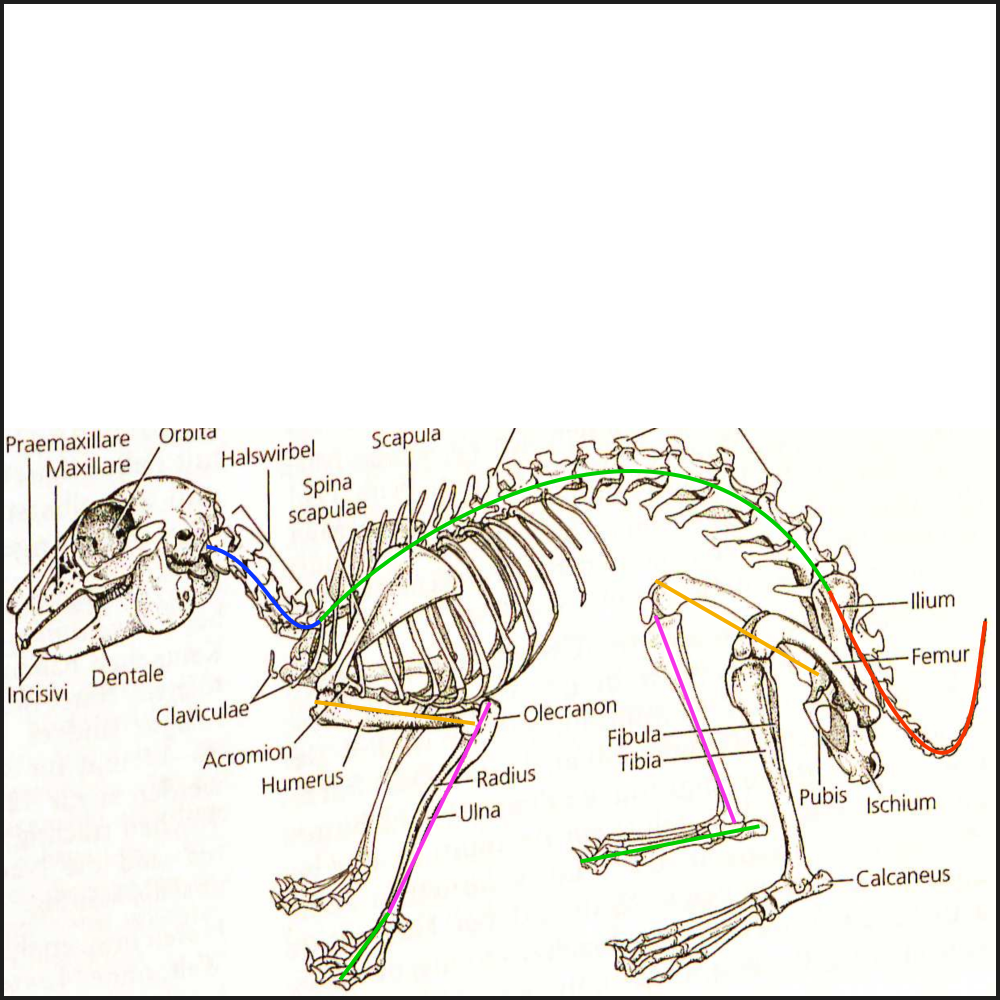
\includegraphics[width=\textwidth]{../../PCA/Skelettbilder/Kaninchen_farbig.png}
  \caption{Annotiertes Skelett eines Kaninchens}
 \end{figure}
 \end{minipage}
\end{frame}


\begin{frame}{Analyse der Eingabedaten}
  \begin{figure}
  \subfloat{\includegraphics[width=0.5\textwidth]{../../PCA/gnuplot_log_weight_with_downscaled_wings_legs_and_weight/results_with_wing_tag/projection_eigenvectors12.pdf}}~
  \subfloat{\includegraphics[width=0.5\textwidth]{../../PCA/gnuplot_log_weight_with_downscaled_wings_legs_and_weight/results_with_leg_tag/projection_eigenvectors12.pdf}}
  
  \caption{Projektion der Eingabedaten auf die Ebene, die durch die erste und zweite Achse des Hyperellipsoids aufgespannt wird.}
 \end{figure}
\end{frame}

\begin{frame}{Mittelwert}
 \begin{figure}
  \centering
  \includegraphics[height=0.6\textheight]{../../PCA/mean_log_weight_downscaled_wings_legs_and_weight(onlyBox,stroke4).jpg}
  \caption{Visualisierung des Mittelwerts der Eingabedaten. Werte, die nicht grafisch visualisiert sind, sind folgende:\\\emph{Flügelpaare} $0{,}159$, \emph{Beinepaare mit Bodenkontakt}~$1{,}39$, \emph{Gewicht} $93$kg}
 \end{figure}
\end{frame}

\begin{frame}{"`Bedeutung"' der Achsen}
 \begin{minipage}{0.6\textwidth}
  \begin{figure}
   \centering
   \subfloat{\includegraphics[height=0.3\textheight]{../../PCA/sqrtEV_log_weight_downscaled_wings_legs_and_weight/EV1_neg.jpg}}
   \qquad
   \subfloat{\includegraphics[height=0.3\textheight]{../../PCA/sqrtEV_log_weight_downscaled_wings_legs_and_weight/EV1_pos.jpg}}
   \\
   \subfloat{\includegraphics[height=0.3\textheight]{../../PCA/sqrtEV_log_weight_downscaled_wings_legs_and_weight/EV2_neg.jpg}}
   \qquad
   \subfloat{\includegraphics[height=0.3\textheight]{../../PCA/sqrtEV_log_weight_downscaled_wings_legs_and_weight/EV2_pos.jpg}}
  \end{figure}
 \end{minipage}~
 \begin{minipage}{0.4\textwidth}
  Koordinaten der visualisierten Datenpunkte in Zeile $i$:
  \begin{itemize}
   \item $i$-te Koordinate: positive \bzw negative Standardabweichung
   \item $j \neq i$: $0$
  \end{itemize}
 \end{minipage}
\end{frame}

%--------------------
\section{Der Algorithmus}
%--------------------
\begin{frame}{Überblick über den Algorithmus}
 \begin{enumerate}
  \setcounter{enumi}{-1}
  \item Benutzereingabe einlesen
  \item PCA auf Beispielskeletten durchführen
  \item[2a.] Punkt $q$ im Konfigurationsraum (zufällig) bestimmen 
  \item[2b.] Parameter für die kontextfreie Grammatik $G$ aus $q$ und Benutzereingabe bestimmen
  \setcounter{enumi}{2}
  \item Bestandteile des Skeletts mit $G$ erzeugen und positionieren
  \item Alle Bestandteile, die nicht auf der Wirbelsäule liegen, spiegeln
  \item 3D-Modell generieren
 \end{enumerate}
\end{frame}

\begin{frame}
  \begin{figure}
   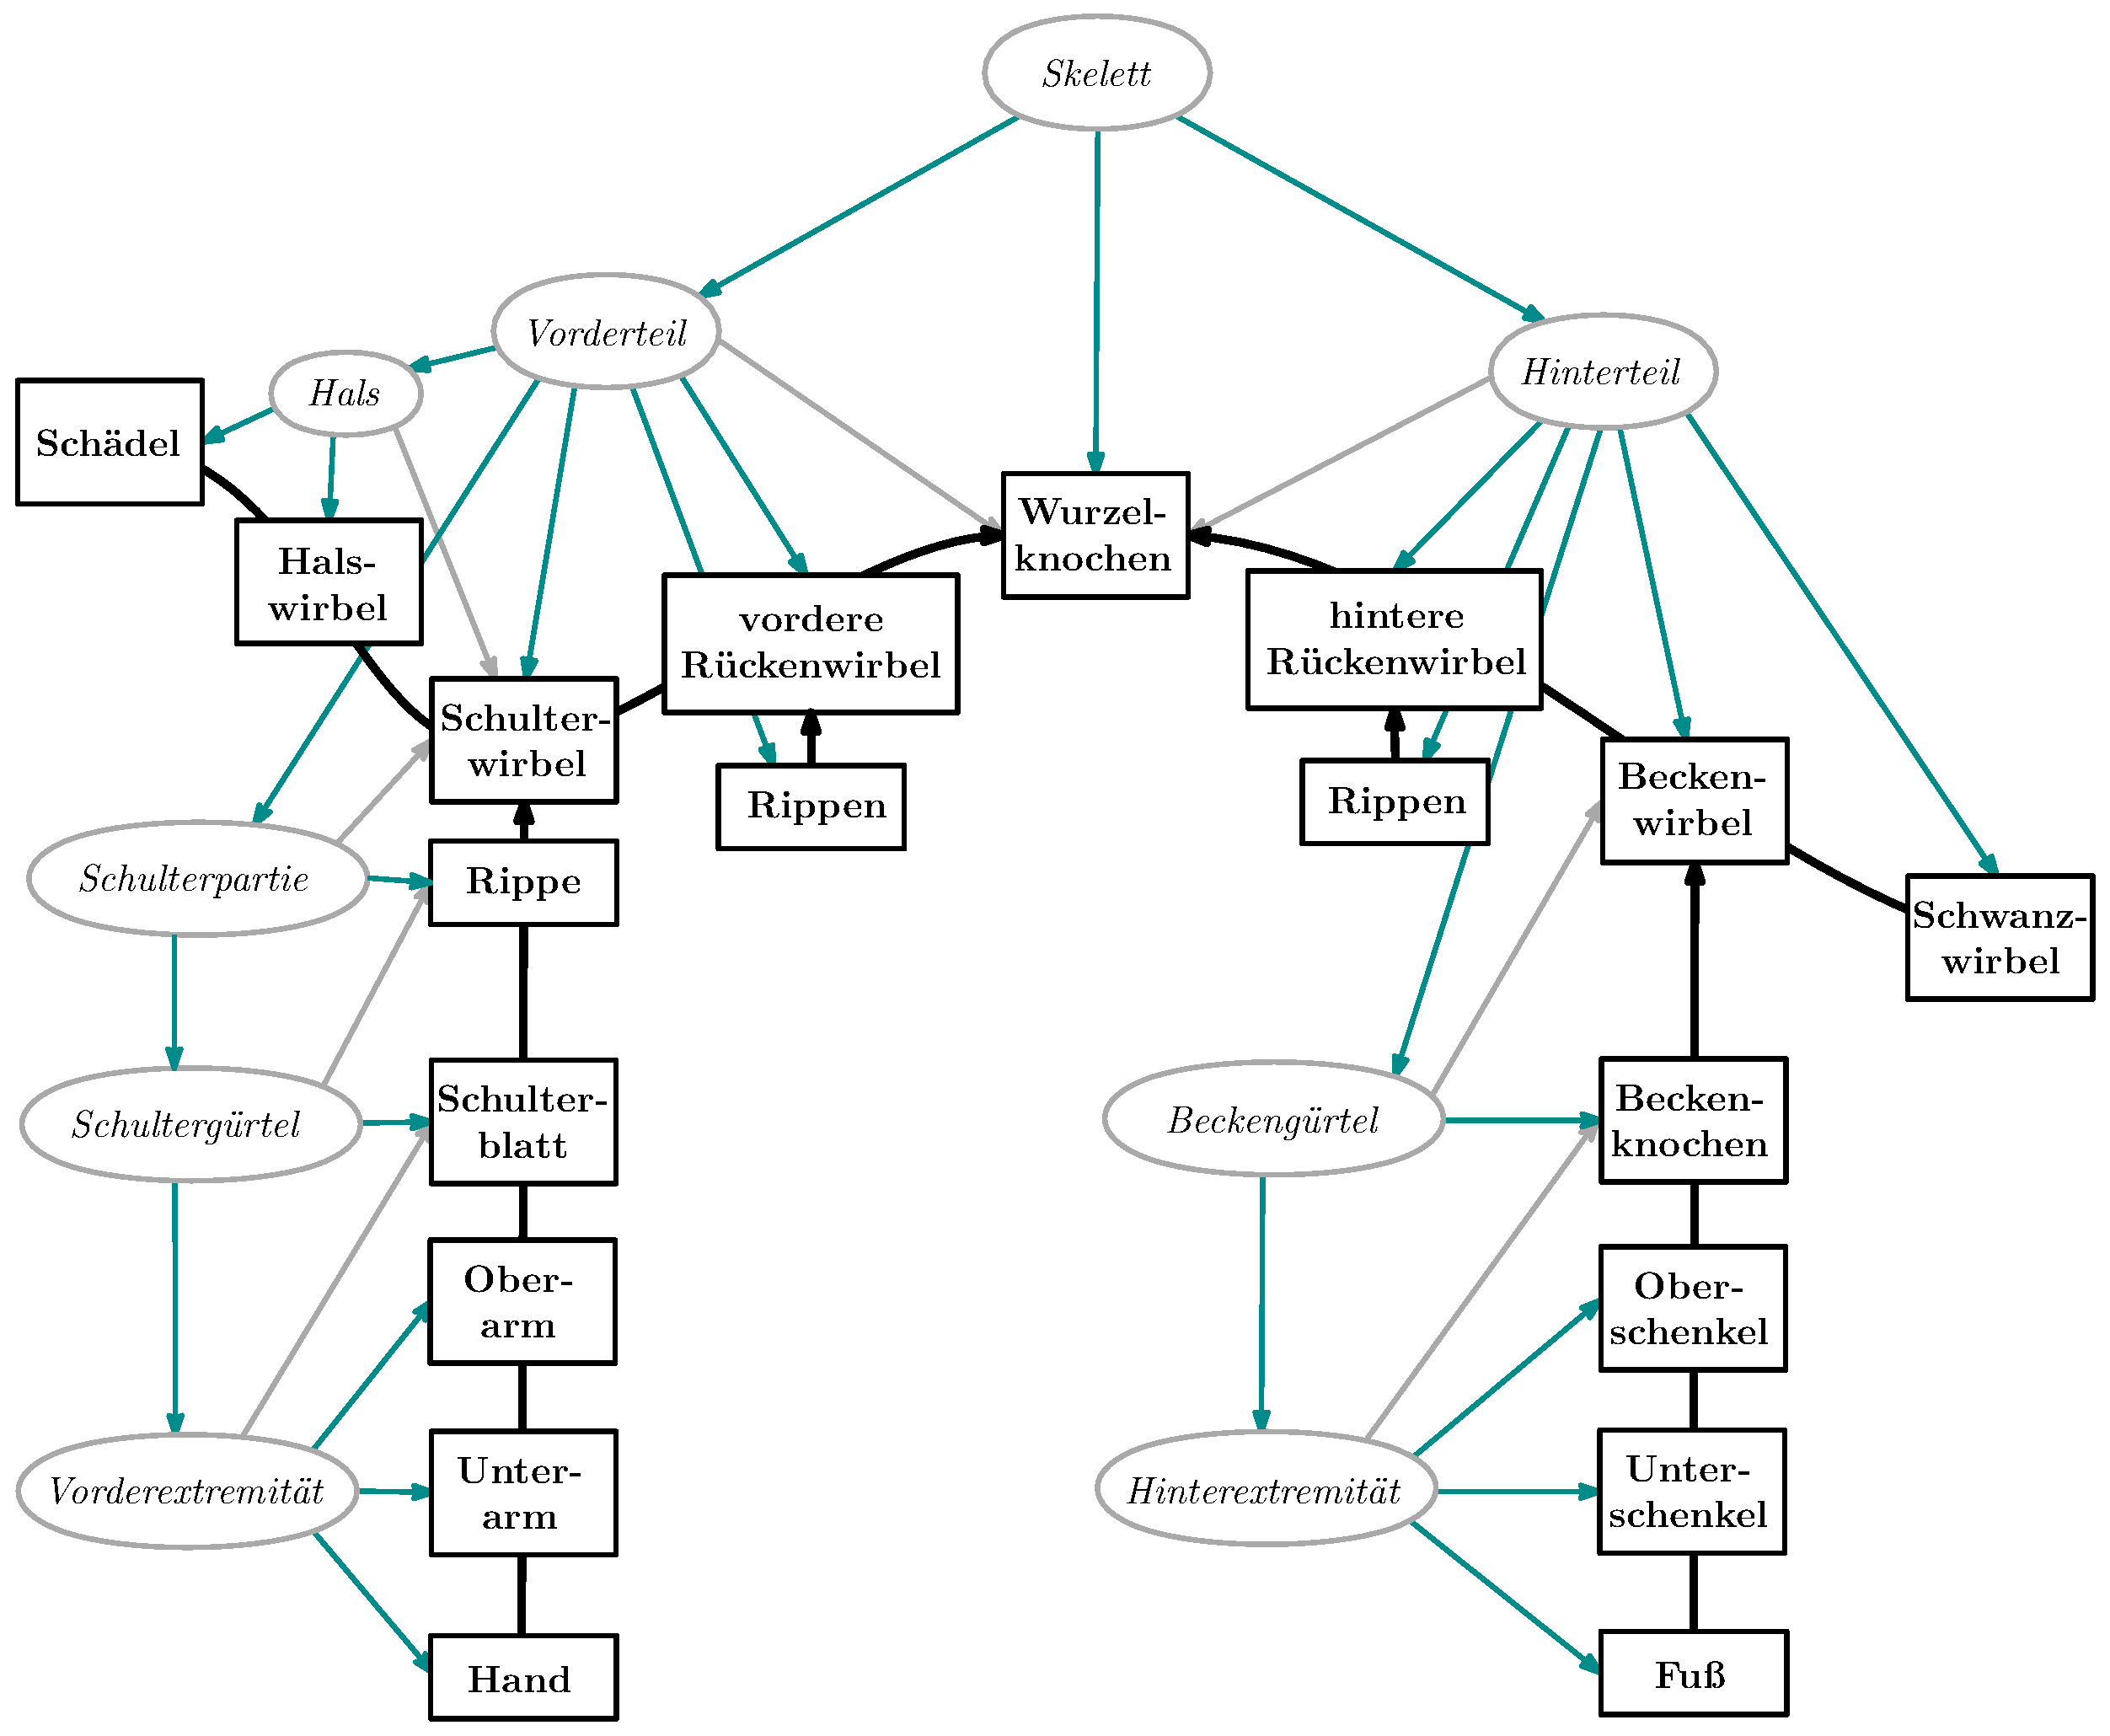
\includegraphics[height=0.9\textheight]{../graphics/grammarGraph_withoutLegend}
  \end{figure}
\end{frame}

\begin{frame}[focus]
 \begin{figure}
  \centering
  \includegraphics[height=0.85\textheight]{../../java_skeleton_generation/example_skeletons/bird.jpg}
  \caption{\scriptsize Als Hintergrund wurde bei allen erzeugten 3D-Modellen \cite{background} verwendet.}
 \end{figure}
\end{frame}

\begin{frame}{Positionierung der Extremitäten}
 \begin{itemize}
  \item Längen der Knochen bekannt
  \item Winkel an Gelenken unbekannt
  \item keine kanonische Ruheposition
  \item Unterscheidung anhand der Funktion:
  \begin{itemize}
   \item Flügel: zufällige Position
   \item Flossen und Arme: ausgerichtet an globalen Achsen
   \item Beine: eigener iterativer Algorithmus
  \end{itemize}
  \item bei Weiterverarbeitung, \zb Animation,\\ wird Positionierung nocheinmal angepasst
 \end{itemize}
\end{frame}

\begin{frame}[focus]
 \begin{figure}
  \centering
  \includegraphics[width=\textwidth]{../../java_skeleton_generation/example_skeletons/fish.jpg}
 \end{figure}
\end{frame}

\begin{frame}[focus]
 \begin{figure}
  \includegraphics[height=0.8\textheight]{../../java_skeleton_generation/example_skeletons/kaenguru.jpg}
 \caption{Känguru}
 \end{figure}
\end{frame}

\begin{frame}[focus]
 \begin{figure}
  \includegraphics[width=\textwidth]{../../java_skeleton_generation/example_skeletons/elefant.jpg}
  \caption{Elefant}
 \end{figure}
\end{frame}

\begin{frame}{Bedingungen}
 \begin{enumerate}
  \item Bedingte Verteilung als Eingabe für PCA
  \begin{itemize}
   \item Anzahl Flügel und Beine
   \item Länge des Halses in $y$-Richtung
   \item Länge des Schwanzes in $x$-Richtung
  \end{itemize}
  \item Vorgegebene Punkte aus Konfigurationsraum laden\\ (\zb Eingabebeispiele)
  \item Schon einmal generierte Skelette laden
 \end{enumerate}
\end{frame}

\begin{frame}{Variationen}
 \begin{block}{Gegeben}
  \begin{itemize}
   \item Punkt $q$ aus dem Konfigurationsraum
   \item generiertes Skelett $S$ (optional)
   \item Benutzereingaben $B$ (optional)
  \end{itemize}
 \end{block}
 
 Vorgehen (statt den Schritten $1+2$ des Algorithmus):
 \begin{enumerate}
  \item zufällig normalverteilten Punkt $q'$ mit Erwartungswert $q$ bestimmen
  \item Parameter $p$ für die Grammatik $G$ aus $q'$ und $B$ und $S$ bestimmen, falls vorhanden
  \item Parameter $p$ variieren (\va Anzahl, Art und Position der Extremitäten)
 \end{enumerate}
\end{frame}


\begin{frame}{Erzeugung eines 3D-Modells}
 \centering
 \includegraphics[width=\textwidth]{../../java_skeleton_generation/example_skeletons/4legs_boxes.jpg}
\end{frame}

%---------------------------
\section{Fantastische Tiere}
%---------------------------

\begin{frame}{Pegasus -- $2$ Extremitätenpaare pro Gürtel}
 \begin{figure}
  \centering
  \includegraphics[height=0.75\textheight]{../../java_skeleton_generation/example_skeletons/pegasus.jpg}
  \caption{Bedingungen: $4$ Beine, $2$ Flügel}
 \end{figure}
\end{frame}

\begin{frame}{Zentaur -- Zweiter Schultergürtel}
 \begin{figure}
  \centering
  \includegraphics[height=0.75\textheight]{../../java_skeleton_generation/example_skeletons/zentaur2.jpg}
  \caption{Bedingungen: $4$ Beine, $2$ Flügel}
 \end{figure}
\end{frame}

\begin{frame}{Ausblick}
 \begin{itemize}
  \item Auch Skelette mit sehr aufrechter Wirbelsäule wie beim Menschen generierbar?
  \item Gewicht der Tiere verwenden \zb als Einfluss auf Größe der Tiere oder Dicke der Knochen
  \item mehr verschiedene und leichter austauschbare Knochenmodelle
  \item interaktiver Algorithmus
  \item Muskeln und Haut generieren
 \end{itemize}
\end{frame}


\begin{frame}[focus]
 Vielen Dank für die Aufmerksamkeit!
 \vfill
 \small weitere Informationen unter \url{https://github.com/Zimmt/skeleton-generation}
\end{frame}

\appendix
\begin{frame}[shrink=5]{Quellen}
 \printbibliography[heading=bibintoc]
\end{frame}

\begin{frame}{Untersuchung auf Normalverteilung}
 Quantil-Quantil-Diagramme
  \begin{figure}
  \subfloat[x-Wert der $3$. Koordinate des Halses]{\includegraphics[width=0.3\textwidth]{../../PCA/gnuplot/results_qq_diagrams/QQ_diagram4.pdf}}~
  \subfloat[Länge der Hand]{\includegraphics[width=0.3\textwidth]{../../PCA/gnuplot/results_qq_diagrams/QQ_diagram24.pdf}}~
  \subfloat[Länge des Oberschenkels]{\includegraphics[width=0.3\textwidth]{../../PCA/gnuplot/results_qq_diagrams/QQ_diagram25.pdf}}
  \phantomcaption
 \end{figure}
\end{frame}

\begin{frame}{Normalverteilung des Gewichts}
 \centering
 \begin{figure}
  \subfloat[linear]{\includegraphics[width=0.3\textwidth]{../../PCA/gnuplot/results_qq_diagrams/QQ_diagram_linear_weight.pdf}}~
  \subfloat[linear (Ausschnitt)]{\includegraphics[width=0.3\textwidth]{../../PCA/gnuplot/results_qq_diagrams/QQ_diagram_linear_weight_without_diagonal.pdf}}~
  \subfloat[logarithmisch]{\includegraphics[width=0.3\textwidth]{../../PCA/gnuplot/results_qq_diagrams/QQ_diagram28.pdf}}
  \phantomcaption
 \end{figure}
 $\Rightarrow$ Das logarithmische Gewicht wird verwendet.
\end{frame}

\begin{frame}{Gewichtung der Merkmale}
 \begin{itemize}
  \item Alle Merkmale zunächst auf $[0, 1]$ skaliert
  \item Diskrete Merkmale (Anzahl Flügel und Beine) nicht normalverteilt, liefern aber hilfreiche Informationen $\rightarrow$ kleiner skalieren
  \item Gewicht nicht Hauptmerkmal $\rightarrow$ kleiner skalieren
 \end{itemize}
\end{frame}

\begin{frame}{Reduzierung der Dimensionalität mit PCA}
  \begin{figure}
  \centering
  \subfloat[Rekonstruktion aus 6 Eigenvektoren]{\includegraphics[width=0.4\textwidth]{../../PCA/animal_reconstructions_log_weight_downscaled_wings_legs_and_weight/6EV/Archaeopteryx_Ausschnitt.jpg}}~
  \subfloat[Eingabebild \cite{Zoologie24Wehner}]{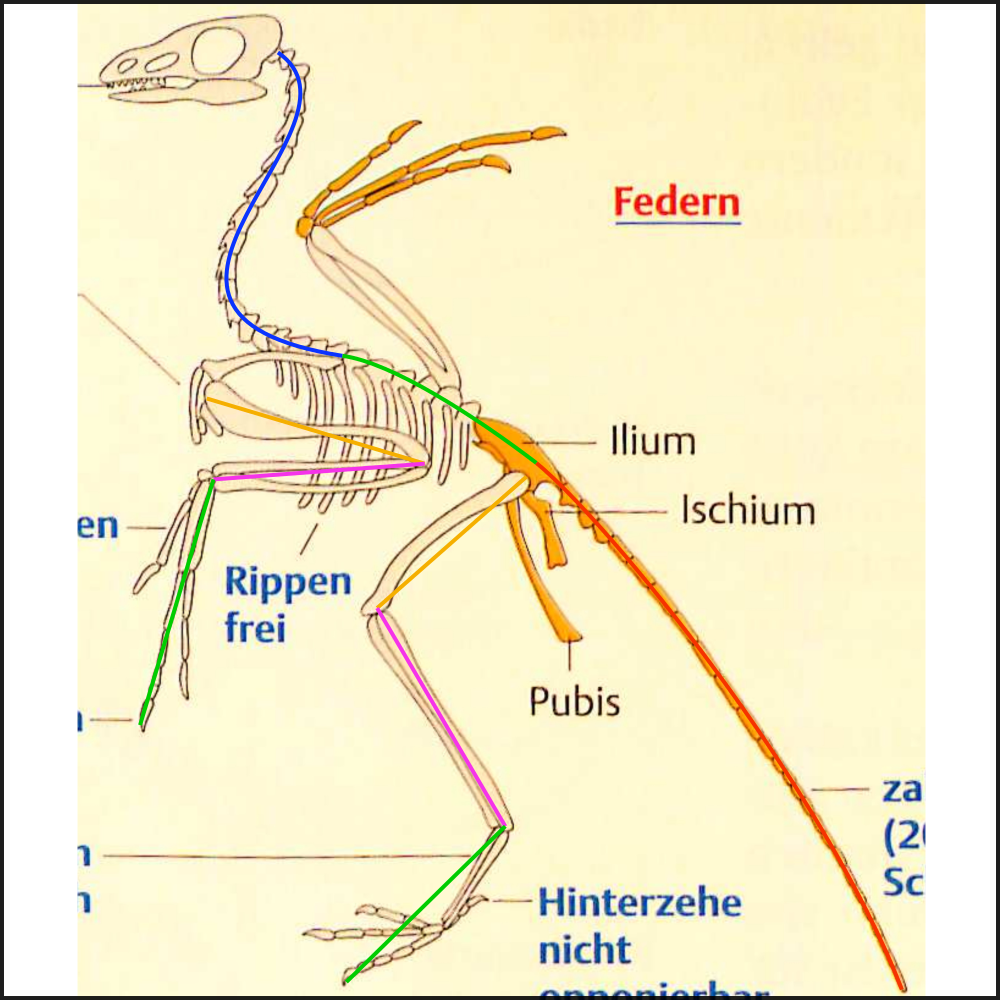
\includegraphics[width=0.4\textwidth]{../../PCA/Skelettbilder/Archaeopteryx_farbig.png}}
  
  \caption{Nicht visualisierte Daten der Rekonstruktion: \emph{Flügel} $0{,}56$, \emph{Beine mit Bodenkontakt} $1{,}594$, \emph{Gewicht}~$94{,}1$kg; Originalwert für das \emph{Gewicht}: $1$kg}
 \end{figure}
\end{frame}

\begin{frame}{Reduzierung der Dimensionalität mit PCA}
 \begin{figure}
  \centering
  \subfloat[Rekonstruktion aus $6$ Eigenvektoren]
  {\includegraphics[width=0.4\textwidth]{../../PCA/animal_reconstructions_log_weight_downscaled_wings_legs_and_weight/6EV/Frosch_Ausschnitt.jpg}}~
  \subfloat[Eingabebild \cite{Spezielle_Zoologie}]{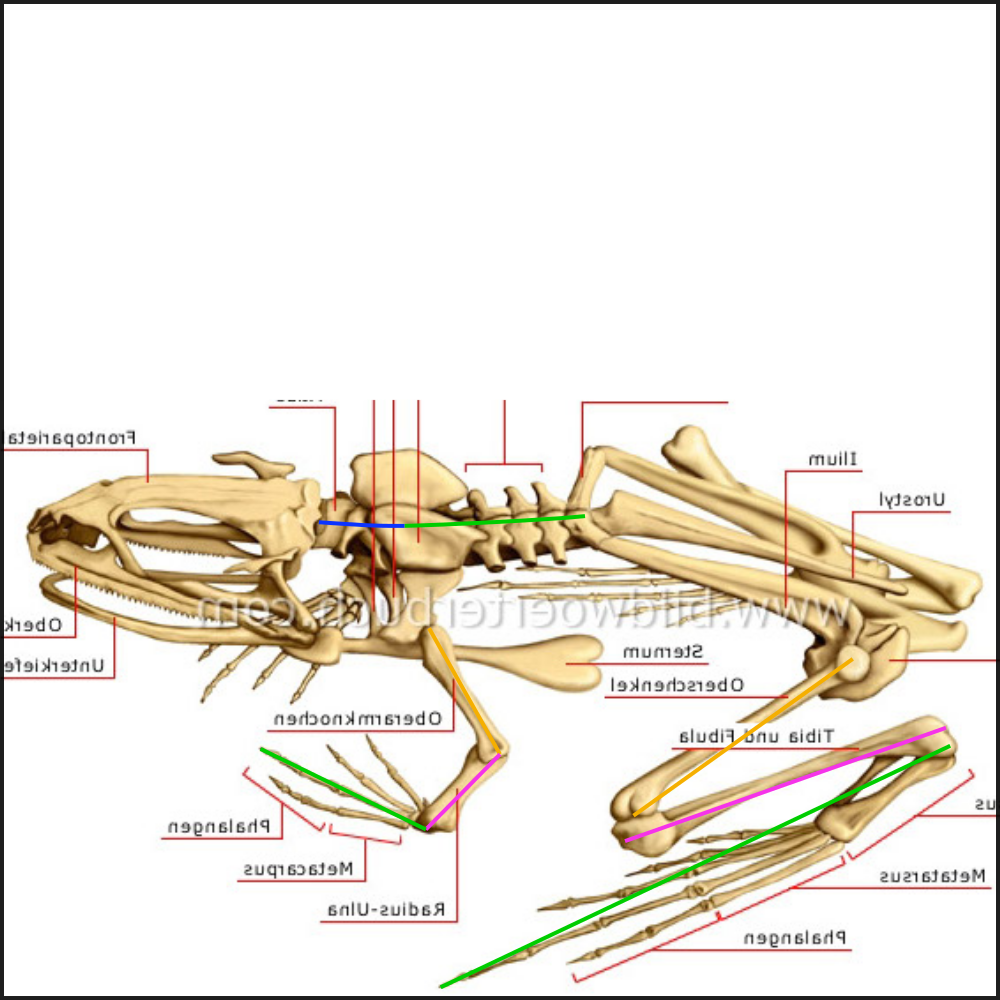
\includegraphics[width=0.4\textwidth]{../../PCA/Skelettbilder/Frosch_farbig.png}}
  
  \caption{Nicht visualisierte Daten der Rekonstruktion: \emph{Flügel} $0{,}4$, \emph{Beine mit Bodenkontakt} $1{,}27$, \emph{Gewicht} $90{,}2$kg; Originalwert für das \emph{Gewicht}: $0{,}01$kg.}
  \label{frosch}
 \end{figure}
\end{frame}



\begin{frame}{Elefant: Vergleich mit dem Originalbild}
 % TODO: ans Ende schieben?
 \begin{figure}
  \subfloat{\includegraphics[width=0.5\textwidth]{../../java_skeleton_generation/example_skeletons/elefant.jpg}}~
  \subfloat{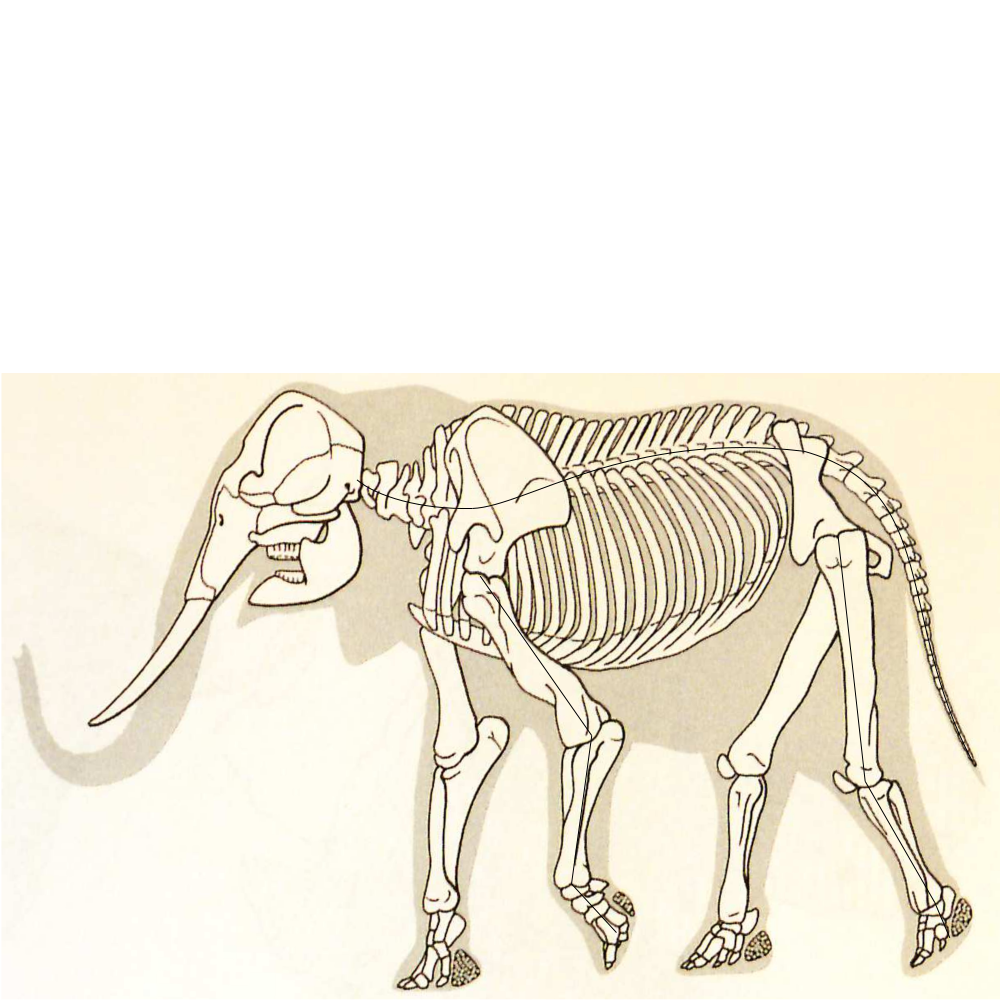
\includegraphics[width=0.5\textwidth]{../../PCA/Skelettbilder/Afrikanischer_Elefant.jpg}}
  \caption{\cite{Spezielle_Zoologie}}
 \end{figure}
\end{frame}

\end{document}
